\documentclass{report}
\usepackage[utf8]{inputenc}    
\usepackage[T1]{fontenc}
\usepackage[francais]{babel}
\usepackage{wrapfig}
\usepackage{graphicx}
\usepackage{listings,xcolor}
\usepackage{appendix}
\usepackage{adjustbox}
\usepackage{titling}
\usepackage{float}
\usepackage{pdfpages}
\usepackage{caption}
\usepackage{subcaption}
\usepackage[hidelinks]{hyperref}
\usepackage{amsmath}
\usepackage{tabto}

\hypersetup{
    colorlinks,
    citecolor=black,
    filecolor=black,
    linkcolor=blue,
    urlcolor=blue
}

%Géométrie des pages
\usepackage{geometry}
\geometry{hmargin=1.9cm,vmargin=1.9cm}

%Définition des couleurs pour le code xml
\definecolor{colorxmlnode}{rgb}{0.2, 0.2, 0.2} 
\definecolor{maroon}{RGB}{178 34 34}


%Profondeur des compteurs et de la tableofcontents
\setcounter{secnumdepth}{3}
\setcounter{tocdepth}{2}


%lst xml
\lstdefinelanguage{XML}
{
  basicstyle=\ttfamily,
  morestring=[s]{"}{"},
  morecomment=[s]{?}{?},
  morecomment=[s]{!--}{--},
  commentstyle=\color{darkgreen},
  moredelim=[s][\color{black}]{>}{<},
  moredelim=[s][\color{red}]{\ }{=},
  stringstyle=\color{blue},
  identifierstyle=\color{maroon}
}


\addto\captionsfrench{%
  \renewcommand\appendixname{Annexe}
  \renewcommand\appendixpagename{Annexes}
}

%Définition des commandes \noeud et \classe
\newcommand\classe[1]{\mbox{\textit{#1}}}
\newcommand\noeud[1]{\textcolor{colorxmlnode}{<\mbox{#1}>}}




\begin{document}

\begin{titlepage}
	\centering
	
    \vspace*{1.2 cm}
    
   	\textsc{\LARGE Master i informatique\\Design Pattern\\[0.3cm]\large Décembre 2017}

	\vspace{2.2cm}
    
    
    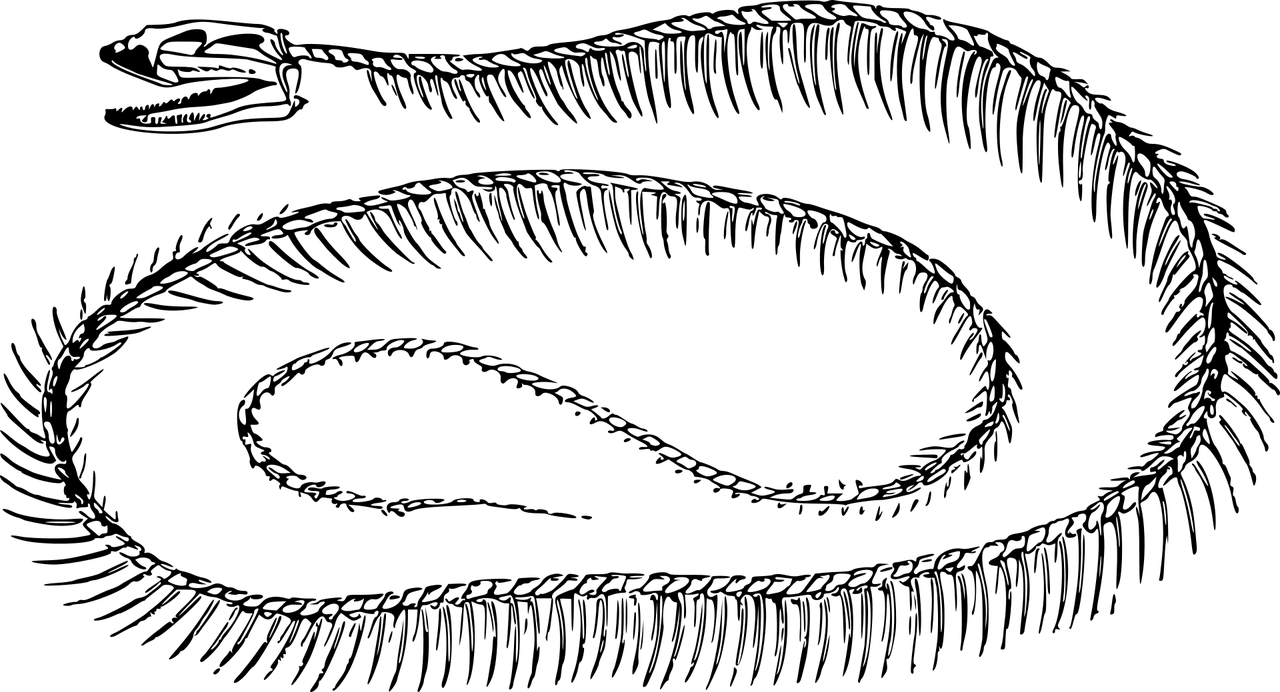
\includegraphics[scale = 0.29]{img/snake.png}\\[0.5 cm]
	\rule{\linewidth }{0.2 mm} \\[0.15 cm]
    {\LARGE \textbf{Projet de Développement}\\[0.2cm] \large
		\textbf{Snake en réseau}}\\
	\rule{\linewidth}{0.2 mm}
       \vspace*{0.1 cm}
	
	\begin{center}
	\vspace{0.3cm}
	
	\emph{Auteurs}\linebreak
	\vspace{0.1cm}
	David \bsc{Dembele}\linebreak
	Alassane \bsc{Diop}\linebreak
	Rahmatou Walet \bsc{Mohamedoun}
		
	\vspace{0.5cm}
	\emph{Professeur}\\
	\vspace{0.1cm}
	Benoit \bsc{Da Mota}
	\end{center}		
	
		
	\vspace{1.5cm}
	\hspace{15cm}
\includegraphics[scale = 0.1]{img/logo.png}

    
    
\end{titlepage}


\tableofcontents

\chapter{Introduction}

	\section{Contexte}
		\par
Dans le cadre de l'UE Design Pattern, de notre premier semestre de Master 1 Informatique à l'Université d'Angers, nous avons poursuivi la phase d'analyse d'un développement de jeu de Snake en réseau. \label{contexte}
	
	\section{Objectifs}
		\par
L'objectif attendu est de permettre à différents joueurs de se connecter au jeu et de jouer entre eux.
Chaque joueur doit disposer d'un serpent qu'il contrôle à l'aide du clavier, avec les touches de direction (HAUT, BAS, GAUCHE, DROITE). Le serpent doit se déplacer pour ramasser des bonus; ces bonus lui permettent de grandir, éventuellement de devenir momentanément invisible, d'augmenter ses points de vie, de faire un retour dans le temps pendant un certains nombre de secondes.\\
Les serpents pourront s'entre-tuer; un serpent tué se transforme en bonus en faveur du serpent tueur ainsi le dernier serpent à survivre sera le gagnant.

\par
Le jeu doit permettre aux joueurs de faire des demandes de connexion et de déconnexion, d'envoyer leurs déplacements au serveur.\\
Le serveur doit gérer les connexions et déconnexions des joueurs et centraliser les actions des joueurs. En effet il gère le plan de jeu partagé par tous les joueurs.\\
À chaque connexion d'un joueur, le serveur doit récupérer les informations du joueur, lui attribuer un serpent, son niveau de compétence et son niveau de jeu.\\
À chaque déplacement d'un serpent, il doit faire une mise à jour du plan de jeu pour prendre en compte la nouvelle position du serpent, en informer les autres joueurs. \label{objectifs}

\chapter{Protocole réseau}
		
	\section{Motivation}
		\par
Dans ce jeu, nous avons utilisé les protocoles TCP\footnote{Transmission Control Protocol (littéralement, « protocole de contrôle de transmissions »), abrégé TCP, est un protocole de transport fiable, en mode connecté. Wikipédia} et UDP\footnote{Le User Datagram Protocol (UDP, en français protocole de datagramme utilisateur) est un des principaux protocoles de télécommunication utilisés par Internet. Il fait partie de la couche transport du modèle OSI, il appartient à la couche 4, comme TCP. Wikipédia}.

\par
Le protocole UDP nous sert dans le cas d'une transmission sans accusé de réception; en effet le protocole UDP repose sur une communication unidirectionnelle. Lorsqu'une machine A envoie un paquet à une machine B, les paquets sont reçus par B sans accusé de réception vers la machine A.

\par
Contrairement au protocole UDP, le protocole TCP repose sur une communication bidirectionnelle. La communication entre deux machines nécessite toujours un accusé de réception du récepteur vers l'émetteur. Dans le cas d'une communication où il faudra limiter la perte de paquet, TCP pourra nous servir. \\ \label{motivation}

	\section{Justification}
		\par
Le protocole UDP est utilisé dans les cas suivants :
\begin{itemize}
	\item déconnexion : lorsqu'un joueur souhaite quitter le jeu il envoie une requête de déconnexion au serveur, le serveur reçoit la requête et lui déconnecte du jeu sans lui en informer (sans accusé de réception).
	
	\item envoi du plan de jeu : lorsque le serveur centralise les actions des utilisateurs, il met à jour le plan du jeu et l'envoie aux joueurs; cette opération peut être répétée autant de fois possible sans perturber le jeu.\\
\end{itemize}
Les informations destinées aux joueurs en provenance du serveur, seront envoyées via le broadcast\footnote{Le broadcast permet au serveur d'envoyer un paquet à tous le joueurs connectés}. \\

\par
Le protocole TCP est utilisé à chaque fois qu'il y ait échange entre le serveur et les joueurs sauf dans le cas d'une déconnexion ou d'un envoi du plan de jeu.\\

Les échanges d'informations entre le serveur et les joueurs se feront via des sockets et doivent être fiables, sans erreurs notamment dans le cas d'une connexion d'un joueur au serveur, de la réception par le serveur des actions des joueurs. 
La communication entre le serveur et les joueurs reposent sur des requêtes HTTP. Ci dessous une représentation de cette communication : 

\begin{figure}[ht]
	\centering
	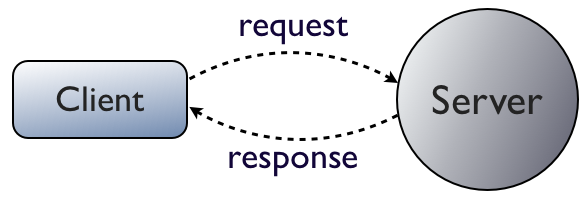
\includegraphics[scale = 0.29]{img/communicationHTTP.png}
	\caption{Communication entre joueur (client) et le serveur}
\end{figure} \label{justification}

	\newpage
	\section{Éventuels problèmes}
		\par
Assurer les communications entre les joueurs et le serveur, en essayant de garantir l'intégrité des paquets, s'avère complexe; des erreurs liées à la transmission des paquets peuvent survenir.\\
En effet, à la fin d'une partie, il peut y avoir un paquet renseignant la position ou le déplacement d'un serpent; si ce paquet arrive après la réception du paquet indiquant la fin de la partie, le joueur émettant le paquet pourrait être bloqué. \\ \label{problemes}
	
	\section{Implémentation}
		\subsection{Le jeu}
			\par

Ci dessous les étapes du déroulement du jeu :

\begin{tabbing}
\hspace{2cm}\=\hspace{1cm}\=\hspace{2cm}\=\kill
 joueur1 \>  --> \>  serveur \> Connexion au serveur \\
 joueur1 \>  --> \>  serveur \> Création d'une nouvelle partie \\
 serveur \>  --> \>  joueurs \> Notification nouvelle partie \\
 joueurs \>  --> \>  serveur \> Participer à la partie \\
 serveur \>  --> \>  joueurs \> Envoie du plan de jeu \\ 
 joueurs \>  --> \>  serveur \> Réception du plan de jeu \\
\end{tabbing} 

 ... Les joueurs commencent à joueur ... \\

\begin{tabbing}
\hspace{2cm}\=\hspace{1cm}\=\hspace{2cm}\=\kill
 joueurX \>  --> \>  serveur \> Participer au jeu \\
 serveur \>  --> \>  joueurX \> Participation acceptée \\
 serveur \>  --> \>  joueurs \> Notification nouveau joueur \\
 joueurY \>  --> \>  serveur \> Remporte la partie \\
 serveur \>  --> \>  joueurs \> Notification partie remportée \\ 
 serveur \>  --> \>  joueurs \> Fin de la partie \\
\end{tabbing}

Au cour du jeu, chaque joueur envoie ses déplacements au serveur qui les centralise et notifie à tous les joueurs qu'ils doivent rafraîchir leur plan de jeu. \\ \label{jeu}
			
		\subsection{Les commandes}
			\par
Les échanges entre le serveur et les joueurs reposent sur la norme ISO-8859\footnote{ISO 8859, également appelée plus formellement ISO/CEI 8859, est une norme commune de l'ISO et de la CEI de codage de caractères sur 8 bits pour le traitement informatique du texte. Wikipédia} qui, a l'avantage d'être connue par tous les systèmes d'exploitation et ne requiert que 8 bits par caractère. \\
8 bits = 1 byte \\

\par
Les commandes des joueurs commenceront par le caractère '/' suivi du nom de la commande. \\
Exemple : \textit{/quit} \\
Cette commande permet à un joueur de quitter une partie de jeu. \\

\par
Toutes les réponses du serveur seront représentées comme suit : 

\begin{itemize}
	\item \textit{1xx} réponse de succès d'une commande
	\item \textit{2xx} réponse d'erreur d'une commande 
	\item \textit{3xx} Commande du serveur \\
\end{itemize}

\newpage
\par
Pour simplifier le transfert de données et éviter des conflits avec le XML (voir \ref{xml}), les caractères suivants ne seront pas acceptés : 

\begin{itemize}
	\item '"' guillemets
	\item '<' signe d'infériorité
	\item '>' signe de supériorité \\
\end{itemize}

Le caractère \textit{' '} (espace) est autorisé, s'il s'agit de séparer des blocs de données. Une commande ou un paramètre ne peut contenir de caractère \textit{' '} (espace). \\

Toutes les commandes devront terminer par le caractère \textbackslash n pour marquer la fin de la commande. \\ \label{commandes}
			
		\subsection{Messages de succès}
			\par

Ci dessous, les messages de succès renvoyés par le serveur : 

\begin{tabbing}

\hspace{5cm}\=\kill
 \textit{100 "Message de bienvenue"}		\> message d'acceptation global \\
 \textit{101 "pseudo" ok} 					\> pseudo accepté \\
 \textit{102 "couleur" "xml"}		 		\> Le joueur de couleur "couleur" rejoint le jeu; "xml" (voir \ref{xml}) représente ses données \\
 \textit{103 "couleur" parti}				\> Le joueur a quitté le jeu \\
 \textit{104 changement niveau}			\> Changement du niveau de jeu dans le serveur \\\\

 \textit{300 debut partie}					\> Commande pour notifier le début de la partie à tous les joueurs \\
 \textit{301 fin "couleur"}				\> Fin de la partie. \textit{"couleur"} désigne le joueur qui remporte la partie. \\
 \textit{302 nbJoueurs {X couleur}}		\> Commande pour envoyer le plan de jeu à tous les joueurs \\

 \textit{303 affichage plan} 				\> Commande pour notifier à tous les joueurs d'afficher le plan de jeu \\
 
\end{tabbing} 
 \label{messagesAcceptes}
			
		\subsection{Messages d'erreur}
			\par

Ci dessous, les messages d'erreur renvoyés par le serveur : 

\begin{tabbing}
\hspace{5cm}\=\kill

 \textit{200 "commande" inconnue} 		\> Le serveur ne connaît pas la commande \\
 \textit{201 format invalide}			\> Le format de la commande n'est pas valide \\
 \textit{202 caractère invalide}		\> Le caractère en question n'est pas accepté (voir \ref{commandes}) \\
 \textit{203 "pseudo" invalide}			\> Le pseudo est déjà utilisé \\
 \textit{204 identification echouee}	\> Le joueur n'a pas encore choisi de pseudo \\
 \textit{205 "pseudo" deja} 			\> Le joueur a déjà un pseudo \\
 \textit{206 "direction" invalide}		\> La direction n'est pas valide (voir \ref{deplacerSerpent}) \\
 \textit{207 "couleur" invalide}		\> La couleur est déjà attribuée à un autre joueur \\
 
\end{tabbing}  \label{messagesRefuses}
			
		\subsection{Les commandes du serveur}
			\par

\begin{itemize}

 \item \textit{300 debut partie}			\tabto{4cm} Commande pour notifier le début de la partie à tous les joueurs
 
 \item \textit{301 fin "couleur"}			\tabto{4cm} Fin de la partie. \textit{"couleur"} désigne le joueur qui remporte la partie. 

 \item \textit{302 nbJoueurs {Xcouleur}}	\tabto{4cm} Commande pour envoyer le plan de jeu à tous les joueurs 

 \item \textit{303 affichage plan} 			\tabto{4cm} Commande pour notifier à tous les joueurs d'afficher le plan de jeu \\
 
\end{itemize}  \label{commandeServeur}		
		
		\subsection{Protocole UDP}
			\par
Le serveur peut être lancé en mode Unicast ou Multicast.\\
En mode Multicast, le serveur envoie de manière automatique les informations, ainsi les joueurs pourront écouter sur le port prévu à cet effet.\\
En mode Unicast, chaque joueur peut demander des informations au serveur qui réponds immédiatement. \label{udp}

		\subsection{Protocole TCP}
			\subsubsection{Joueur vers Serveur}
				\begin{enumerate}
					\item Messages
					\par

\begin{tabbing}
	\hspace{5cm}\=\kill

	\textit{100 "Message de bienvenue"} \>
	Message reçu par le joueur une fois connecté au jeu. \\

	\textit{200 "commande" inconnue} \>
	Lorsque le serveur reçoit une commande qu'il ne connaît pas. \\

	\textit{201 format invalide} \>
	Lorsque le format de la commande n'est pas valide. \\

	\textit{204 identification echouee} \>
	Lorsqu'un client non connecté essaie d'envoyer un message.\\

\end{tabbing} \label{messages}
					\item Nom du joueur
					\par
$/pseudo$ $"pseudojoueur"$
\par
Cette commande permet de définir le pseudo du joueur. Cette commande doit être la première à exécuter par le joueur. À l'exception de la commande $/quit$, toutes les autres commandes sont ignorées jusqu'à ce que le joueur définit son pseudo.\\

Ci dessous les réponses possibles à cette commande : 
\begin{itemize}
	\item 101 pseudo valide.
	
	\item 203 pseudo déjà utilisé.

	\item 210 le joueur a déjà un pseudo.\\
\end{itemize} \label{nomJoueur}
					\item Participer au jeu
					\par
\textit{/join}

\par
Cette commande nécessite permet de participer au jeu.\\

Ci dessous les réponses possibles à cette commande :

\begin{itemize}

	\item \textit{100 "Bienvenue au jeu"} 

	\item \textit{204 "identification echouee"} \\
	Une couleur est attribuée au joueur. Une liste XML\label{xml} lui est envoyée, voir exemple ci-dessous:\\
	
		\textit{102 bleu <joueurs>} \\
			\tabto{1cm} \textit{<joueur pseudo="pseudo" couleur="couleur" score="score" />} \\
			\tabto{1cm}	\textit{...} \\
		\textit{</joueurs>}

\end{itemize}

À chaque fois qu'un joueur rejoigne le jeu, un message est envoyé aux autres joueurs déjà présent dans le jeu, pour leur notifier de sa présence.
\textit{102 "couleur" "xml"} \\ \label{participerJeu}
					\item Quitter le jeu
					
\par
\textit{/quit} \\
Cette commande permet au joueur de quitter le jeu. \\

À chaque fois qu'un joueur quitte le jeu, un message est adressé aux autres joueurs : \\

\textit{103 "couleur" parti} \\
Informer aux autres joueurs restants que le joueur de couleur \textit{"couleur"} a quitté le jeu.
\\ \label{quitterJeu}
					\item Notifier la réception du plan de jeu
					\par

$/receptionPlan$\\
Cette commande notifie au serveur la réception du plan de jeu par un joueur.\\

La commande $/receptionPlan$ ne retourne pas de messages.\\ \label{receptionPlanJeu}
					\newpage
					\item Déplacer le serpent
					\par

\textit{/turn {H | B | G | D}}

\begin{tabbing}
\hspace{1cm}\=\hspace{2cm}\=\kill
G \>  aller à \> gauche \\
D \>  aller à \> droite \\
H \>  aller en \> haut \\
B \>  aller en \> bas
\end{tabbing} 

Ci dessous les réponses possibles à cette commande :
\begin{itemize}
	\item \textit{206 "direction" invalide}
	\item \textit{100 "direction valide"} \\
\end{itemize}
 \label{deplacerSerpent}
					\item Fin de la partie
					\par

$303 ~ fin ~ "couleur"$

Notifier à tous les joueurs que la partie est terminée. $"couleur"$ désigne la couleur du joueur qui remporte la partie. \\ \label{finPartie}
					
				\end{enumerate}				

			\subsubsection{Serveur vers Joueurs}
				\par

Les commandes du serveurs sont envoyés pour notifier un changement d'état; elles ne nécessitent pas de confirmation excepté au début du jeu (voir \ref{envoiPlan}). \\ \label{serveurJoueur}
				
				\begin{enumerate}
					\item Début de la partie
					\par

\textit{300 debut partie} \\

Notifier à tous les joueurs que le jeu a commencé. \\ \label{debutPartie}
					\item Fin de la partie
					\par

$303 ~ fin ~ "couleur"$

Notifier à tous les joueurs que la partie est terminée. $"couleur"$ désigne la couleur du joueur qui remporte la partie. \\ \label{finPartie}
					\item Envoi du plan de jeu
					\par

\textit{302 nbJoueurs {couleur1 ... couleurN}}

\begin{itemize}

	\item \textit{nbJoueurs} 	\tabto{4cm} nombre de joueurs participant au jeu 
	
	\item \textit{couleur1 ... couleurN} 	\tabto{4cm} les couleurs des joueurs participants\\
 
\end{itemize} 

Avant le début de chaque partie, le plan de jeu est envoyé à tous les joueurs. La partie commencera une fois que tous les joueurs auront notifié au serveur la réception du plan de jeu. \\
 \label{envoiPlan}
					\item Affichage du plan de jeu
					\par

\textit{303 affichage plan} \\

Une fois que le serveur aura reçu toutes les notifications de réception du plan de jeu, il ordonne aux joueurs d'afficher le plan de jeu afin qu'ils puissent savoir la position de chaque concurrent. \\ \label{affichePlan}
					\newpage
					\item Nouveau joueur
					\par

\textit{102 "couleur" "xml"}

\begin{itemize}

 \item \textit{"couleur"} 	\tabto{2cm} couleur attribuée au nouveau joueur
 
 \item \textit{"xml"}  		\tabto{2cm} données du nouveau joueur \\

\end{itemize} 

Lorsqu'un nouveau joueur rejoint le jeu, une notification de sa présence est envoyée à tous les autres joueurs déjà présents dans le jeu. \\ \label{nouveauJoueur}
					\item Déconnexion d'un joueur
					\par

\textit{103 "couleur" parti}

\begin{itemize}

	\item \textit{"couleur"} 	\tabto{2cm} couleur du joueur parti 
 
\end{itemize} 

Notifier aux autres joueurs la déconnexion au jeu du joueur de couleur \textit{"couleur"}. \\ \label{joueurParti}
					
				\end{enumerate}			

\chapter{Conception}
			
	\section{Cas d'utilisation}
			\par
Les échanges entre les joueurs et le serveur peuvent être résumés par les cas d'utilisation suivants où les acteurs sont les joueurs : 

\begin{itemize}

	\item Se Connecter
	\item Entrer son nom
	\item Deconnecter
	\item Creer une partie de jeu
	\item Initialiser le jeu
	\item Jouer
	\item Consulter l'aide
	\item Consulter score
	\item Inviter joueur
	\item Quitter le jeu

\end{itemize}

Ci dessous le diagramme des cas d'utilisation : \\

\begin{figure}[ht]
	\centering
	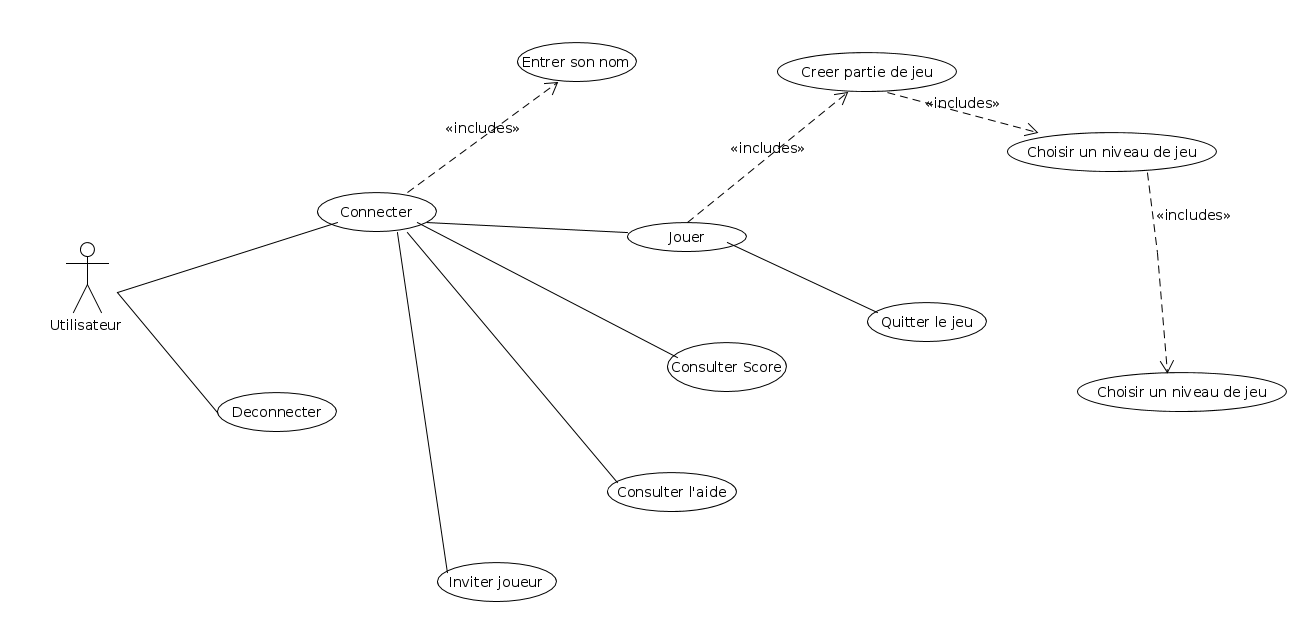
\includegraphics[scale = 0.40]{img/useCase.png}
	\caption{Diagramme des cas d'utilisation}
\end{figure}
 \label{cas_utilisation}

	\newpage			
	\section{Points de changement et d'évolution}
			\par
Durant une partie de jeu, beaucoup d'objets sont amenés à être modifiés. En effet, les actions effectuées par les joueurs entraînent d'états. Ainsi pour un joueur donné, nous pouvons dire que les points de changement concerne : 

\begin{itemize}

	\item le serpent : le comportement du serpent change; il se déplace, ramasse des bonus, s'allonge au fur et à mesure du jeu. Sa visibilité peut changer ainsi que son nombre de vie.
	
	\item le niveau de jeu : à chaque fin de partie, les joueurs peuvent changer de niveau; ils passent d'un niveau inférieur à un niveau supérieur.
	
	\item le plan de jeu : il change en fonction du niveau de jeu. Chaque niveau de jeu propose un plan de jeu différent, plus complexe.
	
	\item le nombre de joueurs : au début du jeu, il y a un nombre de joueurs défini; ce nombre est amené à évoluer positivement si un joueur rejoint la partie et négativement si le serpent d'un joueur meurt.
	
	\item le score : plus un joueur ramasse des bonus, plus son score augmente.
	
	\item l'accès au serveur : l'accès au serveur d'un joueur peut passer d'un état connecté à un état déconnecté et inversement.
	
	\item une partie de jeu : elle peut passer d'un état début à un état en cours, d'un état en cours à un état pause, d'un état en cours à un état terminé.
	
\end{itemize}
 \label{changement}
			\input{Conception/evolution.tex} \label{evolution}
			
	\section{Design envisagé}
			\par
Notre application repose sur une architecture 3-Tiers\footnote{L'architecture trois tiers, aussi appelée architecture à trois niveaux ou architecture à trois couches, est l'application du modèle plus général qu'est le multi-tier. L'architecture logique du système est divisée en trois niveaux ou couches : couche de présentations, couche de traitement, couche d'accès aux données. C'est une architecture basée sur l'environnement client-serveur. Wikipédia.}\\

Cette architecture nous permet de mieux distinguer chaque partie, d'où une conception plus optimale. Ainsi, nous aurons trois parties distinctes : 

\begin{itemize}

	\item couche client (les joueurs) : cette partie regroupe les joueurs qui se connectent au serveur. Nous aurons une abstraction des joueurs physiques, une représentation des joueurs en mémoire du côté de la couche client. Ci dessous le diagramme de classe de la couche client :

\begin{figure}[!h]
	\centering
	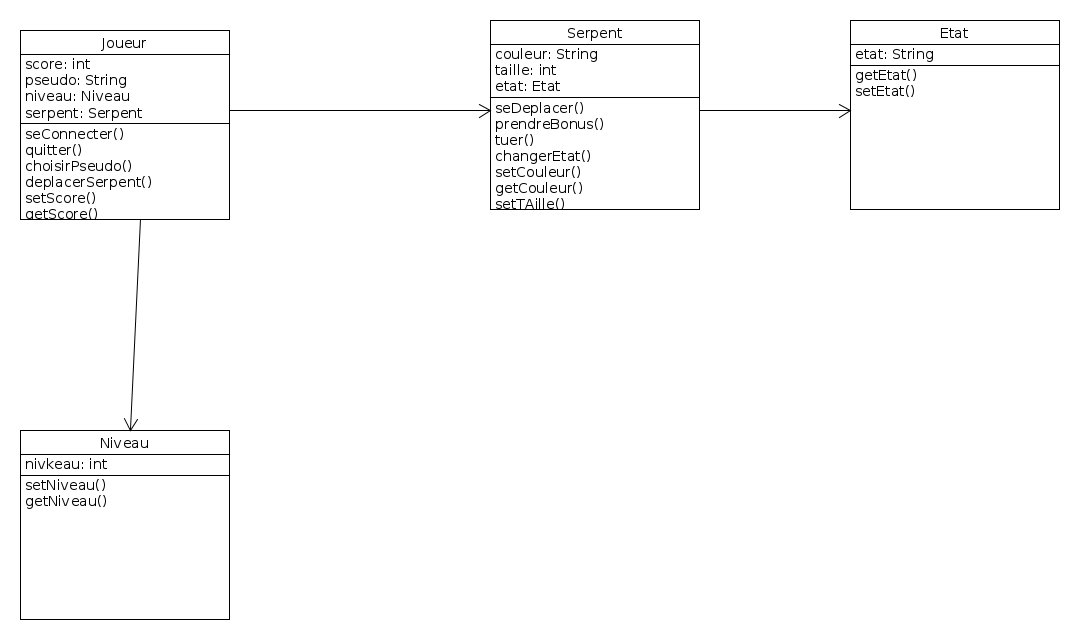
\includegraphics[scale = 0.40]{img/diagClient.png}
	\caption{Diagramme de classe de la couche client}
\end{figure}

	
	\item couche serveur : cette partie regroupe à la fois le serveur, la vue, le modèle (les classes métiers). \\
	Le serveur assure tout ce qui est communication avec les joueurs, centralise leurs actions. Le modèle est une abstraction des joueurs physiques, une représentation des joueurs en mémoire du côté dans la couche serveur. La vue représente le plan, la partie visible qui sera partagée par tous les joueurs, la partie qui permet aux joueurs d'interagir avec le jeu, serveur. \\
	
	Afin de mieux séparer les composants de cette couche, nous structurons cette couche en utilisant le patter MVC, ainsi nous aurons de manière distincte le serveur qui est en même temps le contrôleur, la vue et le modèle. Ci dessous une représentation du pattern MVC :

\begin{figure}[!h]
	\centering
	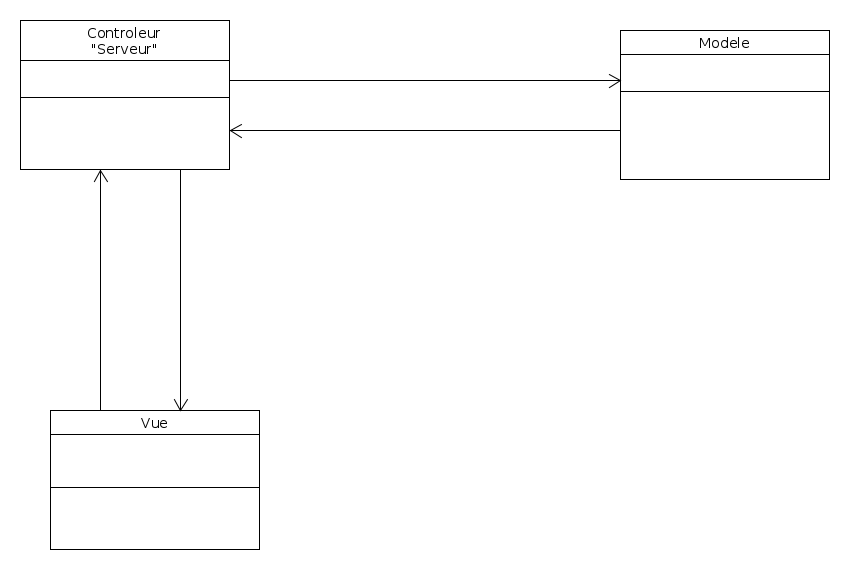
\includegraphics[scale = 0.40]{img/diagMVC.png}
	\caption{Représentation du design pattern MVC}
\end{figure}

	
	Le serveur communique avec la vue et le modèle via le pattern Façade. Ci dessus, le diagramme des classe du pattern MVC intégrant le pattern Façade du serveur :

\begin{figure}[!h]
	\centering
	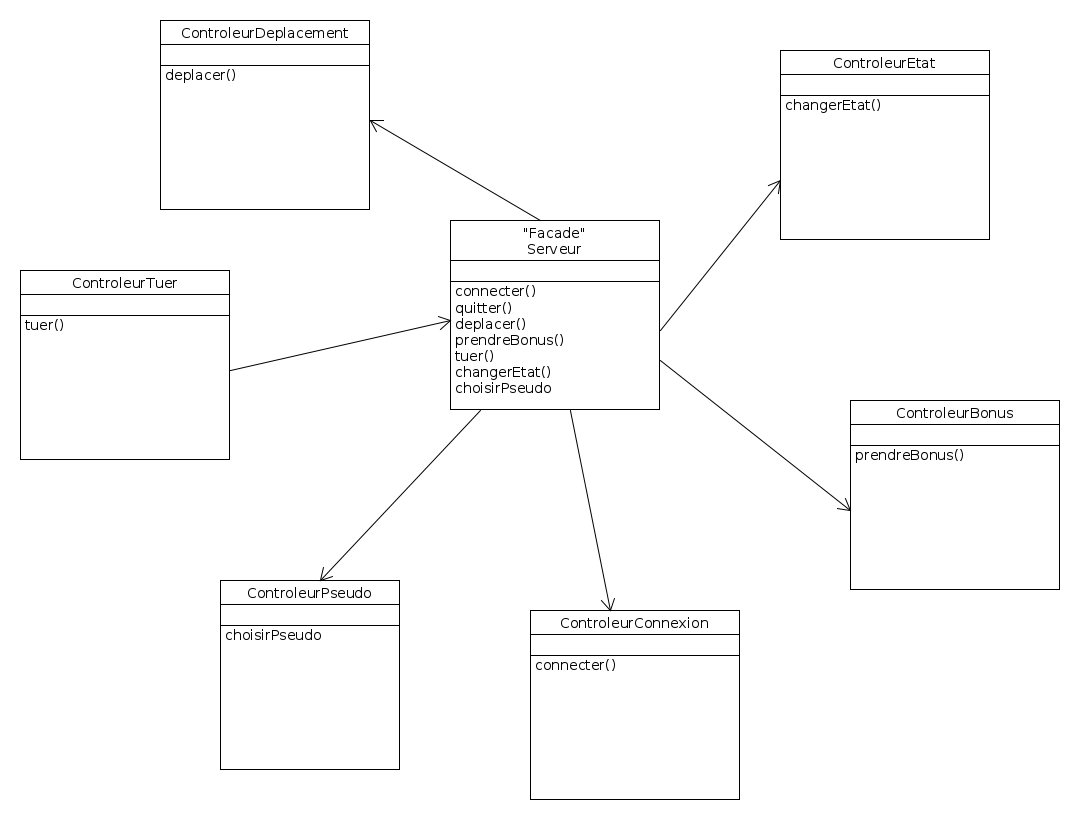
\includegraphics[scale = 0.40]{img/diagServeur.png}
	\caption{Diagramme de classe de la couche serveur}
\end{figure}
\newpage
	
	\item couche persistance : la persistance des données est gérée dans cette partie. \\
	Les données sont une abstraction des joueurs en base de données. Dans cette couche, les données sont des objets des classes métiers. \\
	
\end{itemize}

\par
Pour faire communiquer ces trois couches, nous mettons en place une conception basée sur différents designs patterns. \\

\par
La communication entre la couche client et celle serveur se fera via le pattern Proxy. Ci dessus une représentation de la communication les couches client et serveur :
\begin{figure}[!h]
	\centering
	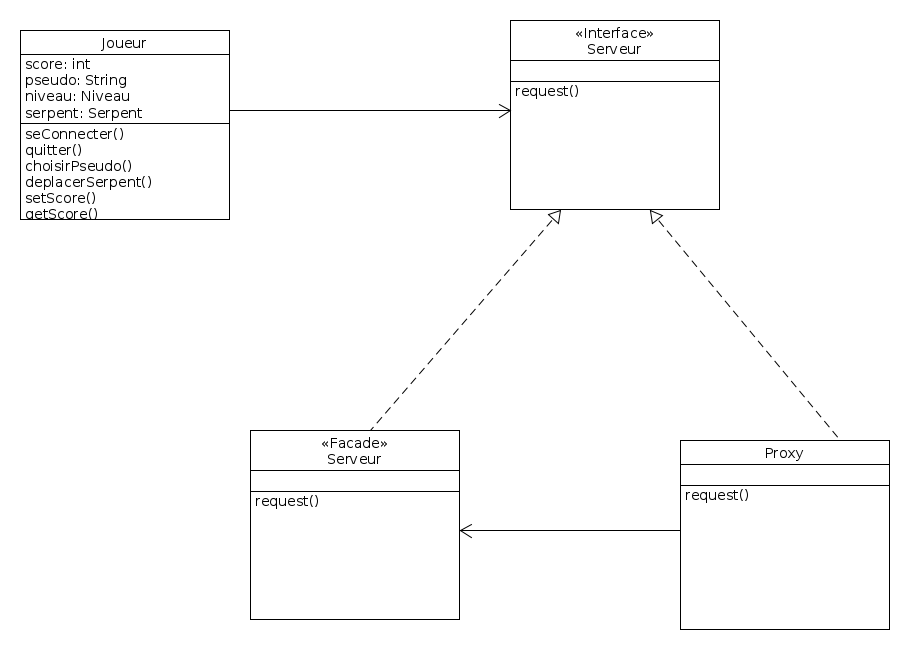
\includegraphics[scale = 0.40]{img/diagProxy.png}
	\caption{Diagramme de classe du pattern Proxy}
\end{figure}
\newpage

\par
La persistance des données passe par le pattern DAO. Ci dessous une représentation de la persistance des données :
\begin{figure}[!h]
	\centering
	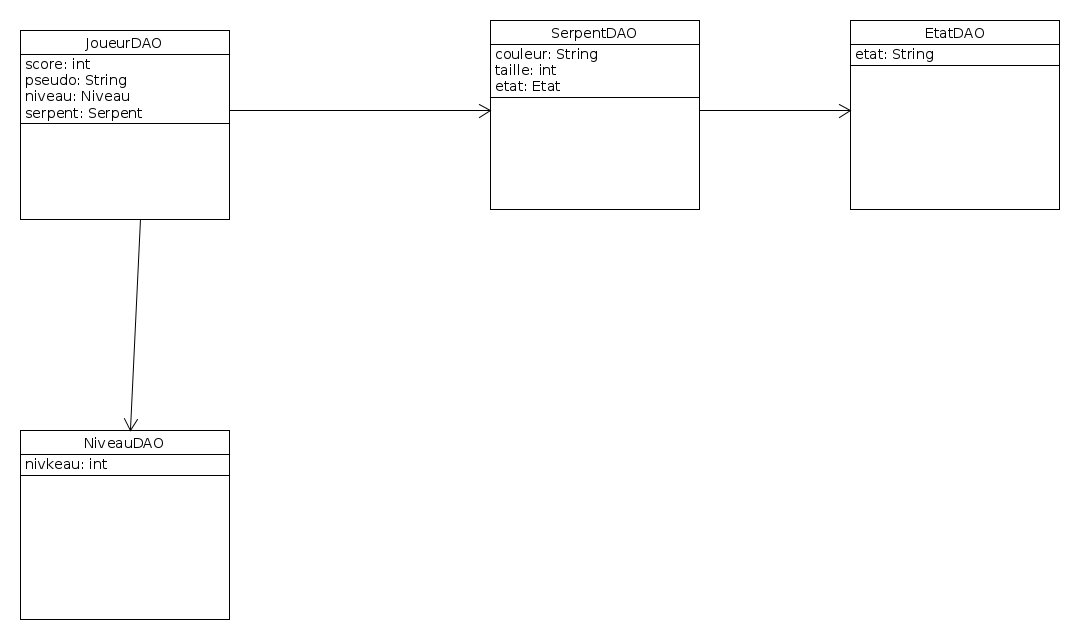
\includegraphics[scale = 0.40]{img/diagDAO.png}
	\caption{Diagramme de classe du pattern DAO}
\end{figure}


 \label{design}
			
	\newpage
	\section{Justification}
			\par
Le protocole UDP est utilisé dans les cas suivants :
\begin{itemize}
	\item déconnexion : lorsqu'un joueur souhaite quitter le jeu il envoie une requête de déconnexion au serveur, le serveur reçoit la requête et lui déconnecte du jeu sans lui en informer (sans accusé de réception).
	
	\item envoi du plan de jeu : lorsque le serveur centralise les actions des utilisateurs, il met à jour le plan du jeu et l'envoie aux joueurs; cette opération peut être répétée autant de fois possible sans perturber le jeu.\\
\end{itemize}
Les informations destinées aux joueurs en provenance du serveur, seront envoyées via le broadcast\footnote{Le broadcast permet au serveur d'envoyer un paquet à tous le joueurs connectés}. \\

\par
Le protocole TCP est utilisé à chaque fois qu'il y ait échange entre le serveur et les joueurs sauf dans le cas d'une déconnexion ou d'un envoi du plan de jeu.\\

Les échanges d'informations entre le serveur et les joueurs se feront via des sockets et doivent être fiables, sans erreurs notamment dans le cas d'une connexion d'un joueur au serveur, de la réception par le serveur des actions des joueurs. 
La communication entre le serveur et les joueurs reposent sur des requêtes HTTP. Ci dessous une représentation de cette communication : 

\begin{figure}[ht]
	\centering
	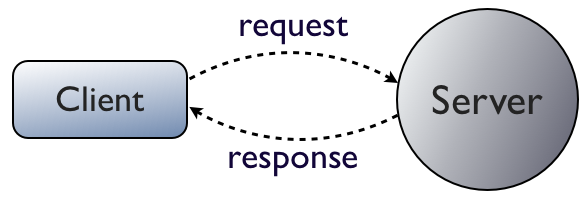
\includegraphics[scale = 0.29]{img/communicationHTTP.png}
	\caption{Communication entre joueur (client) et le serveur}
\end{figure} \label{justification}
			

\chapter{Conclusion}
	\par

Tout au long de cette conception, nous avons essayé de mettre en place des solutions souples et évolutives, qui pourront être facilement maintenables. \\

Cependant, des points restent à développer, à savoir donner aux joueurs la possibilité de créer autant de parties de jeu que possible, de pouvoir inviter d'autres joueurs à rejoindre une partie de jeu, de sauvegarder et restaurer une partie de jeu. \label{conclusion}
\end{document}
